\documentclass[a4paper]{article}

%------------------------------------------------------------
\usepackage[a4paper, total={6in, 9in}]{geometry}
\usepackage{amsmath, amssymb}
\usepackage{booktabs}
\usepackage{caption}
\usepackage{enumitem}
\usepackage{graphicx}
\usepackage{float}
\usepackage{inconsolata}
\usepackage{listings}
\usepackage{mathtools}
\usepackage{pstricks-add}
\usepackage{siunitx}
\usepackage[most]{tcolorbox}
\usepackage{tikz, pgfplots}
\usepackage{epstopdf} %converting to PDF
\usepackage{hyperref}
\usepackage{xfrac}

\usetikzlibrary{shapes.geometric}
\usetikzlibrary{arrows}
\usetikzlibrary{calc}

%------------------------------------------------------------
\graphicspath{{./fig/}}
\pgfplotsset{compat=1.13}
%------------------------------------------------------------
\setlength{\parindent}{0in}

\lstdefinestyle{C++}{
	language=C++,
	basicstyle=\ttfamily,
	keywordstyle=\color{blue}\ttfamily,
	stringstyle=\color{red}\ttfamily,
	commentstyle=\color{green}\ttfamily,
	morecomment=[l][\color{magenta}]{\#},
	showstringspaces=false
}

%------------------------------------------------------------
\newtcblisting[auto counter]{sexylisting}[2][]{sharp corners, 
    fonttitle=\bfseries, colframe=gray, listing only, 
    listing options={basicstyle=\ttfamily,language=C++}, 
    title=Listing \thetcbcounter: #2, #1}

%------------------------------------------------------------
\lstset{language=C++,
        basicstyle=\ttfamily,
        keywordstyle=\color{blue}\ttfamily,
        stringstyle=\color{red}\ttfamily,
        commentstyle=\color{green}\ttfamily,
        morecomment=[l][\color{magenta}]{\#},
        showstringspaces=false
}
%------------------------------------------------------------
\tikzstyle{block} = [draw, fill=blue!20, rectangle, 
    minimum height=3em, minimum width=3em]
\tikzstyle{sum} = [draw, fill=blue!20, circle, node distance=1cm]
\tikzstyle{input} = [coordinate]
\tikzstyle{output} = [coordinate]
\tikzstyle{pinstyle} = [pin edge={to-,thin,black}]

%------------------------------------------------------------
\newlength{\arrow}
\settowidth{\arrow}{\scriptsize$1000$}

\newcommand*{\myrightarrow}[1]{\xrightarrow{\mathmakebox[\arrow]{#1}}}

\newcommand{\uvec}[1]{\boldsymbol{\hat{\textbf{#1}}}}

%------------------------------------------------------------

\begin{document}
\title{ENG252 Dynamics: Project}
\author{Shane Reynolds}
\maketitle

\section{Introduction and Scope}
Torsional springs are capable of storing energy if they are displaced by some angle $\theta$ beyond their resting position. Letting $V_s$ be the energy stored in a torsional spring, and letting $\kappa$ be the torsional spring coefficient, Giancoli \cite{Giancoli:2000} defines the stored energy in a torsional spring as:
\begin{equation}
	V_s = \frac{1}{2} \kappa \theta^2
\end{equation}

The scope of this assignment is to use the stored energy in a mousetrap to move a wheeled vehicle 4.5$\si{\meter}$, deposit a load, and then travel back to the stating point.

\section{Design}
Mechanical design of the vehicle was informed through online research - a popular approach employed a lever arm attached to the mousetrap. The lever arm applies a moment to the drive shaft via tensioned string, causing the wheels to turn as the mousetrap is de-energised. Complete vehicle construction can be seen in Figure 1. Figures 2 and 3 show a detailed view of the string wound onto the drive shaft; and the mousetrap with attached lever arm, respectively. The main alteration to researched designs saw buffers attached to the drive shaft to increase diameter. This allowed larger drive shaft torque on take off for both initial and return legs of vehicle excursion. Increased torque provides greater angular acceleration, yielding increased linear acceleration assuming no wheel slippage. String is wound around the increased diameter drive shaft such that once vehicle velocity is established the string shifts back to the original shaft size ensuring enough drive shaft rotations to traverse the required distance. The drive shaft set up can be seen in Figure 2.

\begin{figure}[h]
	\centering
	\begin{minipage}{0.45\textwidth}
		\centering
		\frame{\includegraphics[height=5cm]{car}}
		\caption{The vehicle is powered by the torsional spring in the mousetrap. A lever arm is attached to the mousetrap which applies a moment to the drive shaft via the string.}
	\end{minipage}
	\hspace{1cm}
	\begin{minipage}{0.45\textwidth}
		\centering
		\captionof{table}{Key vehicle characteristics.}
		\begin{tabular}{p{3cm}rc}
			\toprule
			Measurement & Value & Unit \\
			\midrule
			Chassis Length & & \\
			Chassis Width & & \\
			Chassis Height & & \\
			Mass & 0.180 & $\si{\kilogram}$ \\
			\bottomrule
		\end{tabular}
	\end{minipage}	
\end{figure}

\begin{figure}[h]
	\centering
	\begin{minipage}[t]{0.45\textwidth}
		\centering
		\frame{\includegraphics[height=5cm]{drive_shaft}}
		\caption{The string is wound around the drive shaft of the vehicle. When the string is tensioned the drive shaft experience torque and subsequent angular acceleration.}
	\end{minipage}
	\hspace{1cm}
	\begin{minipage}[t]{0.45\textwidth}
		\centering
		\frame{\includegraphics[height=5cm]{mouse_trap_lever}}
		\caption{The mouse trap has the dowel lever arm fixed to the side of the mouse trap.}
	\end{minipage}
\end{figure}

\begin{figure}[h]
	\centering
	\begin{minipage}[t]{0.45\textwidth}
		\centering
		\frame{\includegraphics[height=5cm]{buffer}}
		\caption{A 3D model of a drive shaft buffer section created using Sketchp.}
	\end{minipage}
	\hspace{1cm}
	\begin{minipage}[t]{0.45\textwidth}
		\centering
		\frame{\includegraphics[height=5cm]{cd_wheel}}
		\caption{Wheels were carefully mounted to the shaft ensuring that the wheel centre of mass aligned with the axis of rotation, achieved using 3D printed mounts.}
	\end{minipage}
\end{figure}

Despite mass increases from the addition of drive shaft diameter buffers, the net result is quicker round trip times. Drive shaft buffers were designed to be removed from shaft to allow for easy experimentation. A 3D model of a buffer section, created in SketchUp, can be seen in Figure 4. Compact Discs (CDs) were used as wheels, fit with rubber balloon sections to the outside for increased traction. It was considered important to mount the wheels to shafts through their centre of mass - not doing this would increase the loss of energy to system vibration. Dowel shaft diameters were less than the size of inner CD holes so a custom mount was created ensure axes of rotation were precisely through the CD centre of mass. Figure 5 shows the CD wheels mounted to the shafts, and Figure 6 shows a 3D model of the wheel mounts created in SketchUp.\\

A further alteration was the inclusion of bearings to reduce rolling friction as the vehicle moves forward. The addition of bearings reduces torsional spring energy being lost to work against the rolling friction forces. Information on the bearings can be found in Figure 9. Bearings were mounted to the vehicle chassis using custom designed mounts shown in Figure 7. Additional information on the bearing mounts can be found in Figure 10. Material choices for vehicle design were informed by a rapid prototyping phase in which many different materials were experimented with including aluminium L sections, timber, and balsa wood for the vehicle chassis. Further, both steel, timber, and balsa shafts were trialled. Finally, moving parts such as pulley systems manufactured with additive manufacturing were trialled too. During this rapid prototyping phase it became apparent that performance was greatly influenced by the amount of mass in the vehicle, given the small amount of energy available in the torsional spring. As a result of these findings, a decision was made to strip away all unnecessary moving parts (such as pulleys), and select only the most light weight materials for construction. Balsa was selected for the main chassis, shown in Figure 8. Timber dowels were chosen for the shafts as a compromise between strength and mass, shown in Figure 12. CDs were selected for wheels, as shown in Figure 11. Lightweight custom plastic parts were designed and created using additive manufacturing where possible.

\vspace{1cm}

\begin{figure}[h]
	\centering
	\begin{minipage}[t]{0.45\textwidth}
		\centering
		\frame{\includegraphics[height=5cm]{cd_mount_design}}
		\caption{Small plastic mounts designed to securely fix the shaft to the Compact Disc wheel at the centre of mass.}
	\end{minipage}
	\hspace{1cm}
	\begin{minipage}[t]{0.45\textwidth}
		\centering
		\frame{\includegraphics[height=5cm]{bearing_mount_design}}
		\caption{Small plastic mounts designed to house the bearings and attach them securely to the vehicle chassis.}
	\end{minipage}
\end{figure}

\vspace{1cm}

\begin{figure}[h]
	\centering
	\begin{minipage}[t]{0.45\textwidth}
		\centering
		\begin{tabular}{p{3.5cm}rc}
			\toprule
			Measurement & Value & Unit \\
			\midrule
			Length & 0.450 & $\si{\meter}$ \\
			Width & 0.010 & $\si{\meter}$  \\
			Mass & 0.006 & $\si{\kilogram}$ \\
			\bottomrule
		\end{tabular}
		
		\vspace{0.5cm}
		
		\frame{\includegraphics[height=5cm]{balsa_frame}}
		\caption{Balsa wood section used for the frame. Two lengths were used.}
	\end{minipage}
	\hspace{1cm}
	\begin{minipage}[t]{0.45\textwidth}
		\centering
		\begin{tabular}{p{3.5cm}rc}
			\toprule
			Measurement & Value & Unit \\
			\midrule
			Diameter & 0.022 & $\si{\meter}$ \\
			Mass & 0.009 & $\si{\kilogram}$ \\
			 & & \\
			\bottomrule
		\end{tabular}
		
		\vspace{0.5cm}
		
		\frame{\includegraphics[height=5cm]{bearing}}
		\caption{Bearings used to reduce friction between shafts and frame.}
	\end{minipage}
\end{figure}


\begin{figure}[h]
	\centering
	\begin{minipage}[t]{0.45\textwidth}
		\centering
		
		\begin{tabular}{p{3.5cm}rc}
			\toprule
			Measurement & Value & Unit \\
			\midrule
			Length & 0.028 & $\si{\meter}$ \\
			Width & 0.028 & $\si{\meter}$ \\
			Mass & 0.002 & $\si{\kilogram}$ \\
			\bottomrule
		\end{tabular}
		
		\vspace{0.5cm}
		
		\frame{\includegraphics[height=5cm]{bearing_mount}}
		\caption{Plastic bearing mounts designed with Sketch up and constructed using additive manufacturing. Four of these were used.}
	\end{minipage}
	\hspace{1cm}
	\begin{minipage}[t]{0.45\textwidth}
		\centering
		
		\begin{tabular}{p{3.5cm}lr}
			\toprule
			Measurement & Value & Unit \\
			\midrule
			Diameter & 0.120 & $\si{\meter}$ \\
			Mass & 0.013 & $\si{\kilogram}$ \\
			 & & \\
			\bottomrule
		\end{tabular}
		
		\vspace{0.5cm}
		
		\frame{\includegraphics[height=5cm]{cd}}
		\caption{Compact disc used for wheels. Four of these were used.}
	\end{minipage}
\end{figure}


\begin{figure}[h]
	\centering
	\begin{minipage}[t]{0.45\textwidth}
		\centering
		\begin{tabular}{p{3.5cm}rc}
			\toprule
			Measurement & Value & Unit \\
			\midrule
			Length (Lever Arm) & 0.400 & $\si{\meter}$ \\
			Length (Shaft) & 0.100 & $\si{\meter}$ \\
			Mass (Lever Arm) & 0.011 & $\si{\si{\kilogram}}$ \\
			Mass (Lever Arm) & 0.003 & $\si{\si{\kilogram}}$ \\
			\bottomrule
		\end{tabular}
		
		\vspace{0.5cm}
		
		\frame{\includegraphics[height=5cm]{dowel}}
		\caption{Dowel lengths used for both the lever arm (one used), and for the shafts (two used) to which wheels were attached.}
	\end{minipage}
	\hspace{1cm}
	\begin{minipage}[t]{0.45\textwidth}
		\centering
		\begin{tabular}{p{3.5cm}rc}
			\toprule
			Measurement & Value & Unit \\
			\midrule
			Length & 0.100 & $\si{\meter}$ \\
			Width & 0.045 & $\si{\meter}$ \\
			Mass & 0.023 & $\si{\kilogram}$ \\
			 & & \\
			\bottomrule
		\end{tabular}
		
		\vspace{0.5cm}
		
		\frame{\includegraphics[height=5cm]{mouse_trap}}
		\caption{Mouse trap used to power vehicle.}
	\end{minipage}
\end{figure}

\clearpage

\section{Machine Dynamics}
\subsection{Theoretical Rolling Friction}

Rolling friction is the friction experienced by a round body when it rolls across a surface \cite{Giancoli:2000}. A rough approximation of the rolling friction coefficient, $\mu_{rf}$, was obtained by placing the vehicle on a flat surface and lifting one end of that surface until the vehicle just starts to move. The experiment set up is shown in Figure 15. Figure 14 shows that if the flat surface length $L$ is known, and the height $h$ is measured just as the vehicle starts to move then $\theta$ can be determined as:
\begin{equation}
	\theta = \arctan \big( \sfrac{h}{L} \big)
\end{equation}
\begin{figure}[h]
	\centering
	\begin{minipage}{0.45\textwidth}
		\centering
		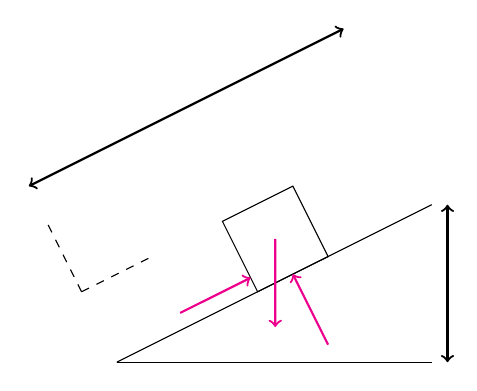
\begin{tikzpicture}
			\draw (0,0) -- (4,0);
			\draw (0,0) -- (4,2);
			\draw[dashed, rotate=26.56] (0,1) -- (1,1);
			\draw[dashed, rotate=26.56] (0,1) -- (0,2);
			\draw[rotate=26.56] (2,0) rectangle (3,1);
			\draw[->, rotate=26.56, thick, color=magenta] (2.5,0.5) -- (2,-0.5);
			\draw[->, rotate=26.56, thick, color=magenta] (1,0.2) -- (2,0.2);
			\draw[->, rotate=26.56, thick, color=magenta] (2.5,-1) -- (2.5,0);
			\draw[<->, thick] (4.2, 0) -- (4.2, 2);
			\draw[<->, thick, rotate=26.56] (0,2.5) -- (4.47,2.5);
		\end{tikzpicture}
		\caption{The horizontal surface is raised on an incline until the point at which the vehicle just begins to move. The include angle and vehicle mass is used to derive an expression for the coefficeint of rolling friction.}
	\end{minipage}
	\hspace{1cm}
	\begin{minipage}{0.45\textwidth}
		\centering
		\frame{\includegraphics[height=5cm]{rolling_friction}}
		\caption{Since bearings were used to reduce rolling friction, the angle of incline is very small as shown here.}
	\end{minipage}
\end{figure}

Assuming the vehicle does not pass through the inclined surface, we note that:
\begin{equation}
	 + \uparrow \sum \boldsymbol{F}_y = 0
\end{equation}

Solving (3) for $F_N$ yields:
\begin{equation}
	F_N = mg \cos \bigg( \arctan \big( \sfrac{h}{L} \big) \bigg)
\end{equation}

Similarly, assuming that the vehicle is on the edge of static equilibrium right before it moves allows us to write:
\begin{equation}
	\stackrel{+}\rightarrow \sum \boldsymbol{F}_x = 0
\end{equation}

Noting that $F{rf} = \mu_{rf} F_N$ we can re-express (5) as:
\begin{equation}
	\mu_{rf} F_N = mg \sin \bigg( \arctan\big( \sfrac{h}{L} \big) \bigg)
\end{equation}

Dividing equation (6) by equation (5) yields:
\begin{equation}
	\mu_{rf} = \frac{h}{L}
\end{equation}

Given the length $L$ was measured at 0.75$\si{\meter}$, and the height $h$ was recorded as $8 \times 10^{-3} \si{\meter}$ the coefficient of rolling friction was calculated as:
\begin{equation}
	\mu_{rf} = 0.011
\end{equation}


\subsection{Spring Coefficient and Potential Energy}
Giancoli defines the moment $M$ created by a torsional spring, for some angle of twist $\theta$ from it's equilibrium position, as:
\begin{equation}
	M = -\kappa \theta
\end{equation} 

We note that $\kappa$ is the spring's torsion coefficient, which is also used to determine the potential energy of a torsional spring according to equation (1). To experimentally determine $\kappa$ for the mousetrap spring, the mousetrap was secured to a bench, and pulley fixed to the trap arm, as shown in Figure 16. Successively greater masses were loaded onto the pulley and the angle $\theta$ was measured for each mass. The pulley redirects the force due to gravity $mg$ so it is orthogonal along the arm of the mousetrap. The moment for each mass loading was calculated using equation (9). The experimental data is presented in Table 2.

\begin{figure}[h]
	\centering
	\begin{minipage}{0.35\textwidth}
		\centering
		\frame{\includegraphics[height=6.5cm]{spring_coeff}}
		\caption{Experimental setup to determine the mousetrap's torsional spring coefficient.}
	\end{minipage}
	\hspace{0.45cm}
	\begin{minipage}{0.55\textwidth}
		\centering
		\captionof{table}{Experimental data captured by loading increasingly larger masses onto the pulley system and measuring the angle of twist from the spring equilibrium position.}
		\begin{tabular}{rrrr}
			\toprule
			Mass $[\si{\kilogram}]$ & Force $[\si{\newton}]$ & Moment $[\si{\newton\meter}]$ & Angle $[\si{\radian}]$ \\
			\midrule
			0.00 & 0.00 & 0.00 & 0.00 \\
			0.09 & 0.84 & 0.03 & 0.15 \\
			0.94 & 0.92 & 0.04 & 0.20 \\
			0.12 & 1.22 & 0.05 & 0.25 \\
			0.22 & 2.18 & 0.09 & 0.52 \\
			0.27 & 2.65 & 0.11 & 0.85 \\
			0.54 & 5.32 & 0.21 & 1.57 \\
			0.61 & 5.95 & 0.24 & 1.89 \\
			0.71 & 7.00 & 0.28 & 2.29 \\ 
			\bottomrule
		\end{tabular}
	\end{minipage}
\end{figure}

\begin{figure}[h]
	\centering
	\begin{tikzpicture}
	\begin{axis}[xlabel=$\theta \ (\si{\radian})$,
	ylabel=$M \ (\si{\newton\meter})$]
	
	\addplot[only marks] coordinates {
		(0.00, 0.00)
		(0.15, 0.03)
		(0.20, 0.04)
		(0.25, 0.05)
		(0.52, 0.09)
		(0.85, 0.11)
		(1.57, 0.21)
		(1.89, 0.24)
		(2.29, 0.28)
	};
	
	\addplot[no marks, blue, domain=0:2.5] {0.13*x};
	
	\end{axis}
	\end{tikzpicture}
	\caption{Angular measurements were plotted against calculated moments in order to determine the torsional spring coefficient. Linear regression was employed to fit a straight line model of equation (9) to the data.}
\end{figure}

Angular measurements were plotted against calculated moments, as shown in Figure 17. Linear regression was used to fit a straight line model, forced through the origin, to the data. We note that this model is is experimentally representative of equation (9), for the torsional spring on the mousetrap. The equation was reported as:
\begin{equation}
	M = 0.13 \ \theta \ \si{\newton\meter}
\end{equation}

We note that the torsion spring coefficient is 0.13 $\si{\newton\meter\per\radian}$

\section{Distance Estimation}

\section{Experimental Performance and Possible Improvements}

\section{Conclusion}

\bibliography{my_bib}
\bibliographystyle{ieeetr}

\end{document}